%%%%%Präambel%%%%%
%Document Style/Page Style
\documentclass[12pt,a4paper]{article}%Schriftgröße, Papierformat einstellen
%\documentclass{scrbook}
\usepackage[top=20mm,bottom=20mm,left=10mm,right=10mm]{geometry}
\usepackage{lipsum}
\usepackage[T1]{fontenc}
\usepackage[ngerman]{babel}
\usepackage[utf8]{inputenc} %für Windows, Linux
\usepackage{titlesec} %improve toc with breaks et cetera
\usepackage{filecontents} %allows to override existing files
\usepackage[nottoc,numbib]{tocbibind}%Add or not add bibliography/index to table of content

%header and footer options
\usepackage{scrlayer-scrpage} %footers and headers
\pagestyle{scrheadings} %style of headers
\clearscrheadfoot %reset everything
\automark[section]{section}
\ofoot{\pagemark}
\ifoot{}
\chead{\headmark}
\setfootsepline{1pt}
\setheadsepline{1pt}
%\setheadsepline[\textwidth+20pt]{0.5pt}

%Citing/Quotation
\usepackage{cite} %improves citation
\usepackage{csquotes}%support for multiple quotation styles
%Pakete laden zur deutschen Rechtschreibung und für Umlaute
\usepackage{harvard} %harvard quotation style
\let\harvardleftorig\harvardleft %option for harvard package

%Symbols
\usepackage[official]{eurosym} %euro symbol
\usepackage{cancel} %diagonal lines for cancelling 
\usepackage{stmaryrd} %St Mary Road symbols for theoretical computer science
\usepackage{units} %set units in typographically correct way
\usepackage{siunitx} %use si units
\usepackage{esvect} %Vectors with arrows
\usepackage{trfsigns} %Transformationszeichen
\usepackage{calc} %adds simple arithmetic functions
\usepackage{amsmath,amssymb,amsthm,amsopn} %mathematic symbols and stuff
\usepackage{bm} %bold symbols in math

%Tables/Environments
\usepackage{longtable} %tables that go more than one page
\usepackage{multirow} %table cell over multiple rows
\usepackage{tabularx} %tabularx environment
\usepackage{booktabs} %provides extra commands for tables
\usepackage{caption} %customise caption in floating environments
\usepackage{array} %use array package
\usepackage{autobreak} %adds line breaking withig align environment
\usepackage{wrapfig} %allows figures or tables to have text wrapped around them
\usepackage{float} %adds options for configuraiton of floationg environments ([H] for example)
\usepackage{hhline} %better horicontal lines

%Misc
\usepackage{graphicx} %optional arguments for includegraphics
\usepackage[dvipsnames]{xcolor} %access to color tones/shades and so on
%\usepackage{subcaption} %test about better image alignment%outdated
\usepackage{subfig}%test about better image alignment

\usepackage{chngcntr} %not quite sure, propably used to specify counting for formulas and stuff
%\usepackage[round]{natbib}
%\usepackage{hyperref}

%Inhaltsverzeichnis mit Links erstellen
\usepackage[colorlinks,
pdfpagelabels,
pdfstartview = FitH,
bookmarksopen = true,
bookmarksnumbered = true,
linkcolor = black,
plainpages = false,
hypertexnames = false,
citecolor = black] {hyperref}

%set depth of toc to specific number
\setcounter{secnumdepth}{4}
\setcounter{tocdepth}{4}

%change how paragraph worls
\titleformat{\paragraph}
{\normalfont\normalsize\bfseries}{\theparagraph}{1em}{}
\titlespacing*{\paragraph}
{0pt}{3.25ex plus 1ex minus .2ex}{1.5ex plus .2ex}

%define subsubsubsection
\newcommand{\subsubsubsection}{\paragraph}

%mainly helping my laziness to flourish

%Makros
%Makro Color
%#1 Text
\def\colBord#1{\begingroup\color{Fuchsia}{#1}\endgroup}
\def\colRed#1{\begingroup\color{Red}{#1}\endgroup}
\def\colGreen#1{\begingroup\color{LimeGreen}{#1}\endgroup}
\def\colBlue#1{\begingroup\color{NavyBlue}{#1}\endgroup}

\def\usGreen#1#2{\underset{\colGreen{#1}}{#2}}
\def\usBord#1#2{\underset{\colBord{#1}}{#2}}

\def\ubGreen#1#2{\underbrace{#2}_{\colGreen{#1}}}

\def\|{\;|\;}
\def\ssum{ \sum_{k=1}^n}

%Some stuff i just dont wanna write everytime
\def\fermi{Fermi-Dirac-Verteilung}
\def\ul#1{\underline{#1}}
\def\€{\euro{}}
\def\epsF{\pmb{\varepsilon}}

\newcommand{\leftRightsection}[2]{
\begin{minipage}[t]{0.5\linewidth}
	\flushleft
	\textbf{#1}
\end{minipage}
	\hfill
\begin{minipage}[t]{0.4\linewidth}
	\flushright
	\textbf{#2}
\end{minipage}
}
\newcommand{\dottedSection}[2]{
\begin{minipage}[t]{0.95\linewidth}
	\textbf{#1 \dotfill #2}
	\end{minipage}
}
%This file contains loosely and not sorted math definitions...

\DeclareMathOperator{\grad}{grad}
\DeclareMathOperator{\diverg}{div}
\DeclareMathOperator{\rot}{rot}
\DeclareMathOperator{\spur}{spur}
\DeclareMathOperator{\determ}{det}

% Umgebungen für Definitionen, Sätze, usw.
\newtheorem{satz}{Satz}[section]
\newtheorem{definition}[satz]{Definition}     
\newtheorem{lemma}[satz]{Lemma}	
\newtheorem{bem}{Bemerkung}[section]
\newtheorem{bsp}{Beispiel}[section]
% Es werden Sätze, Definitionen etc innerhalb einer Section mit
% 1.1, 1.2 etc durchnummeriert, ebenso die Gleichungen mit (1.1), (1.2) ..                  
\numberwithin{equation}{section}


%neue Befehle definieren
\newcommand{\R}{\mathbb{R}} %zB \R als Abkürzung für das Symbol der reellen Zahlen
\newcommand{\N}{\mathbb{N}}
\newcommand{\Z}{\mathbb{Z}}
\newcommand{\Q}{\mathbb{Q}}
\newcommand{\C}{\mathbb{C}}
\newcommand{\diffp}{\partial}
\newcommand{\lapl}{\Delta}
%\def\lapl{\Delta}
%\newcommand{\diverg}{\operatorname{div}}

\def\vecT#1{\left(\begin{array}{c} #1 \end{array}\right)}
\def\dddot{\cdot \\ \cdot \\ \cdot}
\def\vecD#1{\vecT{#1_1 \\ \dddot \\ #1_d}}
\def\vecDt#1#2{\vecT{#1 \\ \dddot \\ #2}}
\def\vecN{\mathcal{O}}
\def\vspan#1{span \lbrace #1 \rbrace}
\def\vdim#1{dim \lbrace #1 \rbrace}
\def\vker#1{ker \lbrace #1 \rbrace}
\def\vrang#1{Rang \lbrace #1 \rbrace}
\def\mzxz#1#2#3#4{\left(\begin{array}{c c} #1 & #2 \\ #3 & #4 \\ \end{array}\right)}
\def\mdxd#1#2#3{\left(\begin{array}{c c c} #1 \\ #2 \\ #3 \end{array}\right)}
\def\dfp#1#2{\frac{\partial #1}{\partial #2}}
\def\diff#1#2{\frac{\mathrm{d}#1}{\mathrm{d}#2}}


\def\inR#1{\qquad ,\; #1 \in \R}
\def\inRs{\in \R}
\def\bracks#1{\left[ #1 \right]}
\def\abs#1{\left| #1 \right|}
\def\brac#1{\left( #1 \right)}
\def\dx{\;dx}
\def\dy{\;dy}
\def\dz{\;dz}
\def\dX{\;d\vec{x}}
\newcommand\citevgl
{\def\harvardleft{(vgl.\ \global\let\harvardleft\harvardleftorig}%
 \cite
}
\newcommand\citeVgl
{\def\harvardleft{(Vgl.\ \global\let\harvardleft\harvardleftorig}%
 \cite
}


\def\ccite#1#2{\glqq #1\grqq\cite{#2}}


\def\ezQu#1{'#1'}

\newcolumntype{L}[1]{>{\raggedleft\let\newline\\\arraybackslash\hspace{0pt}}m{#1}}

\def\multiTwo#1#2{\multicolumn{2}{>{\hsize=\dimexpr2\hsize+2\tabcolsep+\arrayrulewidth\relax}#1}{#2}}
\def\multiThree#1#2{\multicolumn{3}{>{\hsize=\dimexpr3\hsize+4\tabcolsep+2\arrayrulewidth\relax}#1}{#2}}

\newcolumntype{L}[1]{>{\raggedleft\let\newline\\\arraybackslash\hspace{0pt}}m{#1}}
\newcolumntype{R}[1]{>{\raggedright\let\newline\\\arraybackslash\hspace{0pt}}m{#1}}
\newcolumntype{P}[1]{>{\centering\arraybackslash}p{#1}}

\def\formTab#1#2{
\begin{equation}
  \begin{tabularx}{12cm}{R{3cm} l l}
    #1 &: &$#2$
  \end{tabularx}
\end{equation}
}
\newcommand{\formTabL}[3]{
\begin{equation}
  \begin{tabularx}{12cm}{R{3cm} l l}
    #1 &: &$#2$ 
  \end{tabularx}
  \label{eq:#3}
\end{equation}}
\def\formTn{$ \\ $\;$ & $\;$ & $}
\def\formTnQ{$ \\ $\;$ & $\;$ & $\qquad}
\def\formTnQQ{$ \\ $\;$ & $\;$ & $\qquad \qquad}
\def\formTnQQQ{$ \\ $\;$ & $\;$ & $\qquad \qquad \qquad}



%really not sure anymore what this is
\newcommand{\tabitem}{~~\llap{\textbullet}~~}

%settings about equation numbering
\renewcommand{\theequation}{\arabic{section}.\arabic{subsection}
.\arabic{equation}}
%Setzt den equation-Zaehler nach jeder Seite zurueck
%\numberwithin{equation}{subsection}	
\numberwithin{equation}{section}
%\setlength\abovedisplayskip{0pt}

%documentspecific definitions
\newcommand{\ld}{\text{ld}}
\newcommand{\overbar}[1]{\mkern 1.5mu\overline{\mkern-1.5mu#1\mkern-1.5mu}\mkern 1.5mu}

%jetzt beginnt das eigentliche Dokument
\begin{document}
\bibliographystyle{agsm}

\author{}


\null  % Empty line
\nointerlineskip  % No skip for prev line
\vfill
\let\snewpage \newpage
\let\newpage \relax
\title{\underline{NT2 Kurzzusammenfassung} \\ $\;$ \\ $\;$ \\ Florian Leuze}
\date{}
\maketitle
\let \newpage \snewpage
\vfill 
\break % page break


\vspace*{\fill} 
\begin{center}
    \begin{LARGE}
		  \glqq Information is
    \end{LARGE}\\
    \begin{LARGE}
		   the resolution of uncertainty.\grqq
    \end{LARGE}\\
    \begin{large}
      (C. E. Shannon)
    \end{large}
\end{center}
\vspace*{\fill}

\newpage
\tableofcontents

\section*{Versionierung}
\begin{tabular}{|p{2cm}|p{1cm}|p{1.5cm}|p{8.5cm}|}\hline
Datum & Vers. & Kürzel & Änderung \\ \hline
30.08.2019 & 0.1 & FL & Erzeugung Dokument; Erzeugung Inhaltsverzeichnis; Erzeugung Versionierung; Erzeugung Literaturverzeichnis; 1.1-1.8;\\ \hline
01.09.2019 & 0.110 & FL & 1.9 - 1.10 \\ \hline
02.09.2019 & 0.111 & FL & 1.11 \\ \hline
06.09.2019 & 0.112 & FL & 2.1; 2.2; 2.3 \\ \hline
09.09.2019 & 0.2 & FL & 2.3: 2.4; 2.5; 2.6; 2.7 \\ \hline
09.09.2019 & 0.21 & FL & small correction about sectioning \\ \hline
\end{tabular}
\listoffigures


%
%%first chapter damn im too lazy to think about some good notes to put here
\newpage
\section{Grundlagen der Informationstheorie} 
	\section{Notationen}
	\subsection{Charakteristische Funktion}
	Die charakteristische Funktion einer Menge $A \subset \R^n$ ist gegeben durch:
	\begin{equation}
		\textsl{x}_A(x) = 
		\begin{cases}
			1 \qquad, x \in A\\
			0 \qquad, x \in \R^n_{\backslash A}
		\end{cases}
	\end{equation}
	
	Dabei gilt
	\begin{equation}
		\textsl{x}_A \cdot \textsl{x}_B = \textsl{x}_{A \cap B}
	\end{equation}
	
	\subsection{Kartesisches Produkt}
	\begin{equation}
		A \times B = \lbrace (a,b)| a \in A, b \in B \rbrace
	\end{equation}
	
	\subsection{Infimum/Supremum}
	Das Infimum einer Menge ist die größte untere Schranke, das Supremum die kleinste obere Schranke. Schreibweise:
	\begin{align}
		\inf_{x\in A} A \\
		\sup_{x \in B} B
	\end{align}
	\newpage
	\subsection{Randpunkt und Rand}
	Ein Randpunkt $a$ von $A \subset \R^n$ ist ein Punkt $a \in \R^n$ mit
	\begin{align}
		B_\varepsilon (a) \cap A \neq 0\\
		B_\varepsilon (a) \cap A^c \neq 0
	\end{align}
	für alle $\varepsilon > 0$. Der Rand $\partial A$ von $A$ ist die Menge aller Randpunkte.
	  \begin{figure}[H] 
		  \centering
		  \includegraphics[width=0.5\textwidth]{./img/mass_randpunkte.png}
		  \caption{Randpunkte \protect\cite{HM3}}
		  \label{fig:randpunkte}
	  \end{figure}

\subsection{Nützliche Hilfssätze}
	\subsubsection{Reduktionsformel Sinus}
	\begin{equation}
		\int_a^b \sin^n(x) \dx =
\frac{n-1}{n}\int_a^b \sin^{n-2}(x)\dx \quad, a,b \in \frac{\pi}{2} \cdot \Z
	\end{equation}		  
	
		
	
\section{Modulation cosinus-förmiger Träger}
	\subsection{Bandbreite}
\formTab{Basisbandbandbreite für reelle $x(t)$}{B = f_{max}}
\formTab{Bandbreite für komplexe $x(t)$}{B = 2\cdot f_{max}}

\subsection{Einzelimpuls}
Der Einzelimpuls ist gegeben durch
\begin{equation}
	g(t) \cdot T = \lbrace 
		\begin{cases}
		1 & ,\;t = 0\\
		\frac{\sin \left(\frac{\pi t}{T}\right)}{\pi \frac{t}{T}} & ,\;sonst
	\end{cases} \nonumber
\end{equation}
Nach \eqref{eq:fourier_corr_einzelimpuls} ist die Fouriertransformierte
\begin{equation}
	G(f) = \lbrace 
	\begin{cases}
		1 & ,\; |f| \leq \frac{R_S}{2} = \frac{1}{2T}\\
		0 & ,\; sonst
	\end{cases} \nonumber
\end{equation}

\begin{figure}[H]
	\centering
	\subfloat[t-domain]{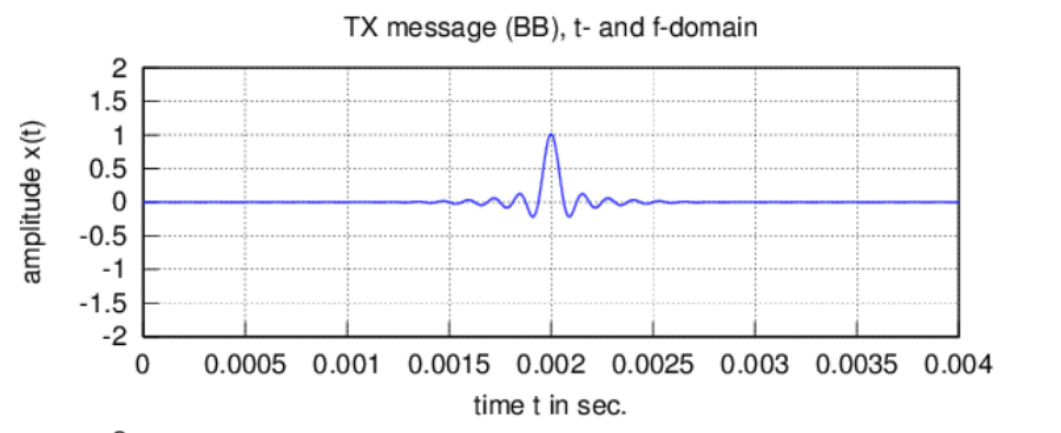
\includegraphics[height=3cm]{./img/mod_einzel_t.png}} ~
	\subfloat[f-domain]{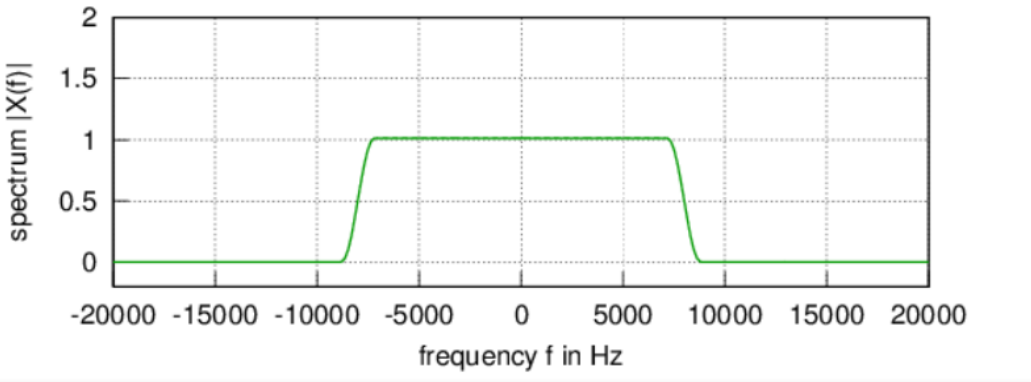
\includegraphics[height=3cm]{./img/mod_einzel_f.png}}
	\caption{Einzelimpuls \protect\cite{NT2}}
\end{figure}

\subsection{Amplitudenmodulation (AM)}
\formTab{Träger}{c(t) = \cos(w_0 t + \varphi_0)}
\formTab{Signal im Passband}{u(t) = \alpha_A \cdot x(t) \cdot c(t) = \alpha_A \cdot x(t) \cdot \cos(w_0 t + \varphi_0) \formTnQQQ = \Re \lbrace \underbrace{x_A \cdot x(t)}_{\text{kompl. Hüllkurve}} \cdot e^{j \varphi_0} \cdot e^{j w_0 t} \rbrace \formTnQQQ = \Re\lbrace x(t) \cdot e^{j w_0 t}\rbrace \quad \text{(für }\varphi = 0 \text{ und  } \alpha_A = 1 \text{)}}
Mit \eqref{eq:fourier_corr_am_1} erhält man durch nutzung der eulerschen Formel
\begin{equation}
	U(w) = \alpha_A \frac{1}{2}\left[X(w+w_0) + X(w-w_0)\right]
\end{equation}

\formTab{Signal mit Offset}{u(t) = \left( x(t) + A_{off} \right) \cdot \cos(w_0 t) \formTnQ = \left( x(t) + A_{off} \right) \left[\frac{1}{2} \cdot e^{j w_0 t} + \frac{1}{2} \cdot e^{-j w_0 t} \right]}
Mit \eqref{eq:fourier_corr_am_off} folgt
\begin{equation}
	x(t) + A_{off} \quad \laplace \quad X(w) + 2\pi A_{off} \delta(w)
\end{equation}

\subsubsection{Frequenzmultiplex}
\formTab{Fourier Identität}{u(t) = \sum\limits_{i=1}^N u_i(t) \quad\laplace\quad U(f) = \sum\limits_{i=1}^N U_i(f)}
\formTab{Kanalraster (bei $\Delta f = const$)}{\Delta f = f_{i+1} - f_i}

\subsubsection{Kohärente Demodulation}
\formTab{Demodulation t-domain}{y(t) = u(t) \cdot \cos(\omega_0 t + \psi) \cdot \beta \formTnQ = u(t) \cdot \cos(\omega_0 t + \psi) \cdot K}
\formTab{Demodulation $\omega$ -/f-domain}{Y(\omega) = \frac{1}{2}X(\omega) \cdot \cos(\psi) \formTn  + \underbrace{\frac{1}{2} X(\omega - 2 \omega_0) \frac{1}{2} \cdot e^{j \psi} + \frac{1}{2} X(\omega + 2 \omega_0) \frac{1}{2} \cdot e^{-j \psi}}_{\text{wird herausgefiltert}}}
\formTab{Typische Normierung}{\alpha_A = \beta = \sqrt{2} \Rightarrow \frac{\alpha_K \beta}{2}=1}
\formTab{Tiefpass Filtereigenschaft}{f_{TP,max} = f_{LP,max} = f_{max,LP} 
\formTnQ f_{max} < f_{max,LP} < 2 f_0 - f_{max}}
\formTab{Orthogonalitätsbedingung}{\psi \neq \frac{\pi}{2} + n \cdot \pi \quad ,\; n \in \Z \quad \text{sonst } v(\omega) = 0} 
\formTab{Identität}{V(\omega) = \frac{1}{2} X(\omega) \cdot \cos(\psi) \quad \formTnQ \laplace \quad v(t) = \frac{1}{2}x(t) \cdot \cos(\psi)}

\subsubsection{Inkohärente Demodulation}
\formTab{Demodulation t-domain}{z(t) = \left[ A_{off} + a(t) \right] \cdot \cos(w_0 t), \; A_{off} + a(t) \overset{!}{>} 0}

\subsection{Quadraturamplitudenmodulation}
Bei der QAM wählt man $x(t) \in \C$ so, dass $X(f)$ asymmetrisch wird und damit die Redundanz der Seitenbänder verschwindet. Es wird ein zusätzlicher Träger der orthogonal zum $\cos$-Träger steht verwendet. Dadurch beeinflussen sich beide Träger nicht.
\formTab{QAM}{u(t) = \alpha_A \left[ x_1(t) \cdot \cos(\omega_0 t) - x_2(t) \cdot \cos(\omega_0 t)\right]} 
Es gilt:
\begin{flalign}
	x(t) = x_{re}(t) + j x_{im}(t) &= x_1(t) + j x_2(t) = x_I (t) + j x_Q(t) + x_N (t) + j x_Q (t) \nonumber \\
	\Rightarrow u(t) &= \Re \lbrace \alpha_A x(t) \cdot e^{j \omega_0 t]} \nonumber \\
	&= \Re \lbrace \alpha_A (x_1 (t) + j x_2 (t)) (\cos(\omega_0 t) + j \cdot \sin(\omega_0 t)) \rbrace \\
	\overset{\alpha_A = 1}{\Rightarrow} u(t) &= x_1(t) \cdot \cos(\omega_0 t) - x_2 (t) \cdot \sin(\omega_0 t)
\end{flalign}
Im Spektrum ergibt sich folglich
\begin{align}
	u(t) &= \Re \left\lbrace \alpha_A x(t) \cdot e^{j \omega_0 t} \right\rbrace \overset{\alpha_A = \sqrt{2}}{=} \frac{\sqrt{2}}{2} \big( x(t) \cdot e^{j \omega_0 t} + \left(x(t) \cdot e^{j \omega_0 t} \right)^* \big) \nonumber\\
	\Rightarrow u(t) \quad &\laplace \quad U(\omega) = \frac{\sqrt{2}}{2} \left( X(\omega - \omega_0) + X^*(-\omega - \omega_0)\right)
\end{align}

\formTab{Demodulation}{v(t) = \beta \cdot u(t) \cdot e^{-j \omega_0 t}}

\subsection{Digitale QAM}
\formTab{Komplexes Symbol}{s_k = s_{k,I} + j s_{k,Q} \quad ,\; s_k \in \frac{1}{\sqrt{2}} \lbrace \pm 1 \pm j \rbrace }
\formTab{Basisbandsignal}{x(t) = \sum\limits_{k=0}^{K-1} s_k g(t-T_s) \quad ,\; T = T_s}
\formTab{Symbolrate}{R_s = \frac{1}{T_s}}
\formTab{Übertragene Bits pro Symbol}{M_b = \ld (M)}
\formTab{Bitrate}{R_b = M_b R_s}

\formTab{Bandbreite (bei Brickstone Impuls)}{B = R_s}
\formTab{Logarithmische Darstellung}{X(f) |_{dB} = 10 \log(X^2(f))}
Das komplexe Basisbandsignal erhält man mit
\begin{align}
	x(t) &= \sum\limits_{k=0}^{K-1} s_k \; g(T-kT_s) = \sum\limits_{k=0}^{K-1} (s_{k,re} + j \; s_{k,im})\;g(t-kT_s) \nonumber\\
	 &= \underbrace{\sum\limits_{k=0}^{K-1} s_{k,re} \; g(t-kT_s)}_{I \in \R} + j\underbrace{\sum\limits_{k=0}^{K-1} s_{k,im}\;  g(t-kT_s)}_{Q \in \R} \quad \in \C
\end{align}

\subsection{Bandbreite für verschiedene $s_k$}
\formTab{Basisbandlage für reelle $s_k$}{B = \frac{1}{2} \; R_s = f_{max}}
\formTab{Basisbandlage für komplexe $s_k$}{B =R_s = 2\cdot f_{max}}
\formTab{Passband für reelle und komplexe $s_k$}{B = R_s =2\cdot f_{max}}

\subsection{Komplexer AWGN Kanal}
\formTab{Kapazität}{C_{AWGN,komplex}(SNR) = 2 \cdot C_{AWGN,reell} (SNR) \formTnQQQ  = \ld (1+SNR)}
\formTab{Rauschleistungsdichte}{N_0 = 2 \sigma^2}
\formTab{Signal-Rausch Abstand}{SNR = \frac{E_s}{N_0}}
 

\newpage
\chapter{Anhänge}
	\subsection{Nachwort}
Dieses Dokument versteht sich einzig als Zusammenfassung des NT2 Stoffes auf Basis der Literatur und der Vorlesungsunterlagen aus der NT2 Vorlesung von Prof. Dr.-Ing Stephan ten Brink. Der Sinn ist einzig mir selbst und meinen Kommilitonen das studieren der Nachrichtentechnik zu erleichtern. In diesem Sinne erhebe ich keinerlei Anspruch auf das hier dargestellte Wissen, da es sich in großen Teilen nur um Neuformulierungen aus der Literatur, den Vorlesungen und aus der Begleitübung. Sollten sich einige Fehler eingeschlichen haben (was sehr wahrscheinlich ist) würde ich mich freuen, wenn man mich per Email (f.leuze@outlook.de) kontaktieren und mir entsprechende Fehler mitteilen würde.

%\nocite{*}
\bibliography{./bib/lit}

\end{document}
